%%%%%%%%%%%%%%%%%%%%%%%%%%%%%%%%%%%%%%%%%%%%%%%%%%%%%%%%%%%%%%%%%%
%%%%%%%% ICML 2014 EXAMPLE LATEX SUBMISSION FILE %%%%%%%%%%%%%%%%%
%%%%%%%%%%%%%%%%%%%%%%%%%%%%%%%%%%%%%%%%%%%%%%%%%%%%%%%%%%%%%%%%%%

% Use the following line _only_ if you're still using LaTeX 2.09.
%\documentstyle[icml2014,epsf,natbib]{article}
% If you rely on Latex2e packages, like most moden people use this:
\documentclass{article}

% use Times
\usepackage{times}
% For figures
\usepackage{graphicx} % more modern
%\usepackage{epsfig} % less modern
\usepackage{subfigure} 
\graphicspath{{figures/}}

% For citations
\usepackage{natbib}

% For algorithms
\usepackage{algorithm}
\usepackage{algorithmic}
\usepackage{amsmath}
\usepackage{amsfonts}
% As of 2011, we use the hyperref package to produce hyperlinks in the
% resulting PDF.  If this breaks your system, please commend out the
% following usepackage line and replace \usepackage{icml2014} with
% \usepackage[nohyperref]{icml2014} above.
\usepackage{hyperref}
\usepackage{color}
\usepackage{soul}
\usepackage{multicol}

% Packages hyperref and algorithmic misbehave sometimes.  We can fix
% this with the following command.
\newcommand{\theHalgorithm}{\arabic{algorithm}}

% Employ the following version of the ``usepackage'' statement for
% submitting the draft version of the paper for review.  This will set
% the note in the first column to ``Under review.  Do not distribute.''
%\usepackage{icml2015} 
% Employ this version of the ``usepackage'' statement after the paper has
% been accepted, when creating the final version.  This will set the
% note in the first column to ``Proceedings of the...''
\usepackage[accepted]{icml2015}


% The \icmltitle you define below is probably too long as a header.
% Therefore, a short form for the running title is supplied here:
\icmltitlerunning{Massively Parallel Methods for Deep Reinforcement Learning}

\begin{document} 

\twocolumn[
\icmltitle{Massively Parallel Methods for Deep Reinforcement Learning}

% It is OKAY to include author information, even for blind
% submissions: the style file will automatically remove it for you
% unless you've provided the [accepted] option to the icml2014
% package.
\icmlauthor{Arun Nair, Praveen Srinivasan, Sam Blackwell, Cagdas Alcicek, Rory Fearon, Alessandro De Maria, Vedavyas Panneershelvam, Mustafa Suleyman, Charles Beattie, Stig Petersen, Shane Legg, Volodymyr Mnih, Koray Kavukcuoglu, David Silver}
{  \\ \{arunsnair, prav, blackwells, cagdasalcicek, roryf, ademaria, darthveda, mustafasul, cbeattie, svp, legg, vmnih, korayk, davidsilver @google.com \}}
\icmladdress{Google DeepMind, London}

% You may provide any keywords that you 
% find helpful for describing your paper; these are used to populate 
% the "keywords" metadata in the PDF but will not be shown in the document
\icmlkeywords{reinforcement learning, deep learning}

\vskip 0.3in
]

\newcommand{\argmax}[1]{\underset{#1}{\operatorname{argmax}}\;}
\newcommand{\argmin}[1]{\underset{#1}{\operatorname{argmin}}\;}
\renewcommand{\max}[1]{\underset{#1}{\operatorname{max}}\;}
\renewcommand{\min}[1]{\underset{#1}{\operatorname{min}}\;}
\newcommand{\expect}[2]{\mathbb{E}_{#1} \left[ #2 \right]}
\newcommand{\TODO}[1]{\hl{TODO: #1}}

\begin{abstract} 
We present the first massively distributed architecture for deep reinforcement learning. This architecture uses four main components: parallel actors that generate new behaviour; parallel learners that are trained from stored experience; a distributed neural network to represent the value function or behaviour policy; and a distributed store of experience. We used our architecture to implement the Deep Q-Network algorithm (DQN)~\cite{mnih2013atari}. Our distributed algorithm was applied to 49 games from Atari 2600 games from the Arcade Learning Environment, using identical hyperparameters. Our performance surpassed non-distributed DQN in 41 of the 49 games and also reduced the wall-time required to achieve these results by an order of magnitude on most games.
\end{abstract} 


\section{Introduction}
\label{sec:intro}

Language modeling is among the important problems that require modeling long-term dependency, with successful applications such as unsupervised pretraining~\citep{dai2015semi,peters2018deep,radford2018improving,devlin2018bert}.
However, it has been a challenge to equip neural networks with the capability to model long-term dependency in sequential data.
Recurrent neural networks (RNNs), in particular Long Short-Term Memory (LSTM) networks~\citep{hochreiter1997long}, have been a standard solution to language modeling and obtained strong results on multiple benchmarks.
Despite the wide adaption, RNNs are difficult to optimize due to gradient vanishing and explosion~\citep{hochreiter2001gradient}, and the introduction of gating in LSTMs and the gradient clipping technique~\citep{graves2013generating} might not be sufficient to fully address this issue.
% ,pascanu2012understanding
Empirically, previous work has found that LSTM language models use 200 context words on average~\citep{khandelwal2018sharp}, indicating room for further improvement.

On the other hand, the direct connections between long-distance word pairs baked in attention mechanisms might ease optimization and enable the learning of long-term dependency~\citep{bahdanau2014neural,vaswani2017attention}.
Recently, \citet{al2018character} designed a set of auxiliary losses to train deep Transformer networks for character-level language modeling, which outperform LSTMs by a large margin.
Despite the success, the LM training in~\citet{al2018character} is performed on separated fixed-length segments of a few hundred characters, without any information flow across segments.
As a consequence of the fixed context length, the model cannot capture any longer-term dependency beyond the predefined context length.
In addition, the fixed-length segments are created by selecting a consecutive chunk of symbols without respecting the sentence or any other semantic boundary.
Hence, the model lacks necessary contextual information needed to well predict the first few symbols, leading to inefficient optimization and inferior performance.
We refer to this problem as \textit{context fragmentation}.

%However, the context length is fixed to hundreds of characters and thus it is not possible to model longer-term dependency. Moreover, it is not clear how the model performs on word-level language modeling data, as the granularity changes.

% Moreover, using auxiliary losses brings additional challenges such as properly tuning the mixture weights and the loss decay schedule.

To address the aforementioned limitations of fixed-length contexts, we propose a new architecture called Transformer-XL (meaning extra long).
We introduce the notion of recurrence into our deep self-attention network. In particular, instead of computing the hidden states from scratch for each new segment, we reuse the hidden states obtained in previous segments.
The reused hidden states serve as memory for the current segment, which builds up a recurrent connection between the segments.
As a result, modeling very long-term dependency becomes possible because information can be propagated through the recurrent connections.
Meanwhile, passing information from the previous segment can also resolve the problem of context fragmentation.
More importantly, we show the necessity of using relative positional encodings rather than absolute ones, in order to enable state reuse without causing temporal confusion.
Hence, as an additional technical contribution, we introduce a simple but more effective relative positional encoding formulation that generalizes to attention lengths longer than the one observed during training.

Transformer-XL obtained strong results on five datasets, varying from word-level to character-level language modeling.
Transformer-XL is also able to generate relatively coherent long text articles with \textit{thousands of} tokens (see Appendix \ref{sec:gen}), trained on only 100M tokens.
% Transformer-XL improves the previous state-of-the-art (SoTA) results from 1.06 to 0.99 in bpc on enwiki8, from 1.13 to 1.08 in bpc on text8, from 20.5 to 18.3 in perplexity on WikiText-103, and from 23.7 to 21.8 in perplexity on One Billion Word.
% Transformer-XL improves the previous state-of-the-art (SoTA) results to 0.99 in bpc on enwiki8, 1.08 in bpc on text8, 18.3 in perplexity on WikiText-103, and 21.8 in perplexity on One Billion Word.
% On small data, Transformer-XL also achieves a perplexity of 54.5 on Penn Treebank without finetuning, which is SoTA when comparable settings are considered.

Our main technical contributions include introducing the notion of recurrence in a purely self-attentive model and deriving a novel positional encoding scheme. These two techniques form a complete set of solutions, as any one of them alone does not address the issue of fixed-length contexts. Transformer-XL is the first self-attention model that achieves substantially better results than RNNs on both character-level and word-level language modeling.

% On WikiText-103, Transformer-XL improves the previous state-of-the-art (SoTA) results from 33 perplexity to 24, with a relative reduction of 27\%. On enwiki8 character-level language modeling, Transformer-XL achieves a SoTA bpc of 1.03, which outperforms \cite{al2018character} by 0.03 with 60+\% fewer parameters. Given a more common model size with 40+M parameters, Transformer-XL achieves a bpc of 1.06, compared to 1.11 by \cite{al2018character}. Transformer-XL also achieves perplexities of 54.5 on Penn Treebank and 29.4 on One Billion Word, which are SoTA when comparable settings are considered.

% Due to the ability of modeling long-range context, our best model uses attention lengths of 1,600 and 3,800 on WikiText-103 and enwiki8 respectively. We also devise a metric called \textit{Relative Effective Context Length} (RECL) that aims to fairly compare the ability of long-range dependency modeling.
% % perform a fair comparison of the gains brought by increasing the context lengths for different models.
% In this setting, Transformer-XL learns a RECL of 900 words on WikiText-103, while the numbers for recurrent networks and Transformer are only 500 and 128.

% We use two methods to quantitatively study the effective lengths of Transformer-XL and the baselines. Similar to \cite{khandelwal2018sharp}, we gradually increase the attention length at test time until no further noticeable improvement ($\sim$0.1\% relative gains) can be observed. Our best model in this settings use attention lengths of 1,600 and 3,800 on WikiText-103 and enwiki8 respectively.
% %In addition, since the effective context length of Transformer-XL can be longer than the attention length due to our recurrent formulation, we devise a metric called \textit{Relative Effective Context Length} (RECL) that aims to perform a fair comparison of the gains brought by increasing the context lengths for different models.
% In addition, we devise a metric called \textit{Relative Effective Context Length} (RECL) that aims to perform a fair comparison of the gains brought by increasing the context lengths for different models.
% In this setting, Transformer-XL learns a RECL of 900 words on WikiText-103, while the numbers for recurrent networks and Transformer are only 500 and 128.

\paragraph{3D Object Detection from RGB-D Data} Researchers have approached the 3D detection problem by taking various ways to represent RGB-D data.

\emph{Front view image based methods:} ~\cite{chen2016monocular, mousavian20163d, xiang2015data} take monocular RGB images and shape priors or occlusion patterns to infer 3D bounding boxes. ~\cite{li2016vehicle, deng2017amodal} represent depth data as 2D maps and apply CNNs to localize objects in 2D image. In comparison we represent depth as a point cloud and use advanced 3D deep networks (PointNets) that can exploit 3D geometry more effectively.

\emph{Bird's eye view based methods:} MV3D~\cite{cvpr17chen} projects LiDAR point cloud to bird's eye view and trains a region proposal network (RPN~\cite{ren2015faster}) for 3D bounding box proposal. However, the method lags behind in detecting small objects, such as pedestrians and cyclists and cannot easily adapt to scenes with multiple objects in vertical direction.
%Our method shares the idea with~\cite{cvpr17chen} in reducing 3D search cost by 2D search first. What differentiates our method from \cite{cvpr17chen} is that, \hao{???} instead of projecting point cloud to images costing loss in 3D geometry, we directly apply PointNet to point clouds that correspond to the 2D regions. % Besides, our method and MV3D can potentially be combined in the bird's eye setting. 3D proposals from our frustum-based PointNet and MV3D can be combined and our 3D network can also be used for bounding box estimation for point cloud in the bird's eye 2D region.

\emph{3D based methods:} ~\cite{wang2015voting, song2014sliding} train 3D object classifiers by SVMs on hand-designed geometry features extracted from point cloud and then localize objects using sliding-window search. \cite{engelcke2017vote3deep} extends ~\cite{wang2015voting} by replacing SVM with 3D CNN on voxelized 3D grids. \cite{ren2016three} designs new geometric features for 3D object detection in a point cloud. \cite{song2016deep, li20163d} convert a point cloud of the entire scene into a volumetric grid and use 3D volumetric CNN for object proposal and classification. Computation cost for those method is usually quite high due to the expensive cost of 3D convolutions and large 3D search space.
%In comparison, we use 2D region proposals from RGB images to reduce the search space from the entire 3D scenes into 3D frustums. Since the points cloud in the frustums have largely varying depth ranges and can be very sparse, it's not applicable to apply CNN on bird's eye view or apply 3D CNN in grids. Our frustum-based PointNet, on the other hand, suits well for this type of data and is able to accurately estimate 3D bounding box with good efficiency.
Recently, \cite{lahoud20172d} proposes a 2D-driven 3D object detection method that is similar to ours in spirit. However, they use hand-crafted features (based on histogram of point coordinates) with simple fully connected networks to regress 3D box location and pose, which is sub-optimal in both speed and performance. In contrast, we propose a more flexible and effective solution with deep 3D feature learning (PointNets).
%In addition we also get 3D instance segmentation as intermediate outputs. Evaluated on SUN-RGBD we show our method is \emph{8.9\%} better than theirs in mAP and \emph{34x} faster at the same time.


% \begin{enumerate}
%     \item ZOOX~\cite{mousavian20163d} image based
%     \item Vote3Deep~\cite{engelcke2017vote3deep} 3d cnn. Recent LIDAR-based methods place 3D windows in 3D voxel grids to score the point cloud
%     \item Voting for Voting~\cite{wang2015voting} Recent LIDAR-based methods place 3D windows in 3D voxel grids to score the point cloud. apply SVM classifers on 3D grids encoded with geometry features
%     \item MV3D~\cite{cvpr17chen}
%     \item VeloFCN~\cite{li2016vehicle} apply convolutional networks to the front view point map in a dense box prediction scheme
%     \item 3DOP~\cite{chen20153d} image based. reconstructs depth from stereo images and uses an energy minimization approach to generate 3D box proposals, which are fed to an R-CNN [10] pipeline for object recognition
%     \item Mono3D~\cite{chen2016monocular} image based. shares the same pipeline with 3DOP, it generates 3D proposals from monocular images.
%     \item 3DFCN~\cite{li20163d} 3d cnn.
%     \item 3DVP~\cite{xiang2015data} introduces 3D voxel patterns and employ a set of ACF detectors to do 2D detection and 3D pose estimation
%     \item Are Cars just 3D Box?~\cite{zeeshan2014cars} fit model to image patch
%     \item ~\cite{zia2013detailed} fit model to image patch
% \end{enumerate}
% \begin{enumerate}
%     \item SlidingShapes~\cite{song2014sliding} apply SVM classifers on 3D grids encoded with geometry features
%     \item DeepSlidingShapes~\cite{song2015sun} 3d cnn.
%     \item 2D-driven~\cite{lahoud20172d}
%     \item ~\cite{deng2017amodal} rgb-d images
%     \item COG feature~\cite{ren2016three}
%     \item Align 3D model in RGB-D~\cite{gupta2015aligning}
% \end{enumerate}

\paragraph{Deep Learning on Point Clouds}
Most existing works convert point clouds to images or volumetric forms before feature learning. \cite{wu20153d, maturana2015voxnet, qi2016volumetric} voxelize point clouds into volumetric grids and generalize image CNNs to 3D CNNs. ~\cite{li2016fpnn, riegler2016octnet, wang2017cnn, engelcke2017vote3deep} design more efficient 3D CNN or neural network architectures that exploit sparsity in point cloud.
However, these CNN based methods still require quantitization of point clouds with certain voxel resolution.
Recently, a few works~\cite{qi2017pointnet,qi2017pointnetplusplus} propose a novel type of network architectures (PointNets) that directly consumes raw point clouds without converting them to other formats. While PointNets have been applied to single object classification and semantic segmentation, our work explores how to extend the architecture for the purpose of 3D object detection.
%!TEX root = gorila_paper.tex
\section{Background}
\subsection{DistBelief}
DistBelief~\cite{dean2012distbelief} is a distributed system for training large neural networks on massive amounts of data efficiently by using two types of parallelism.
Model parallelism, where different machines are responsible for storing and training different parts of the model, is used to allow efficient training of models much larger than what is feasible on a single machine or GPU.
Data parallelism, where multiple copies or replicas of each model are trained on different parts of the data in parallel, allows for more efficient training on massive datasets than a single process.
We briefly discuss the two main components of the DistBelief architecture -- the central parameter server and the model replicas.

The central parameter server holds the master copy of the model. The job of the parameter server is to apply the incoming gradients from the replicas to the model and, when requested, to send its latest copy of the model to the replicas. The parameter server can be sharded across many machines and different shards apply gradients independently of other shards.

Each replica maintains a copy of the model being trained. This copy could be sharded across multiple machines if, for example, the model is too big to fit on a single machine. The job of the replicas is to calculate the gradients given a mini-batch, send them to the parameter server, and to periodically query the parameter server for an updated version of the model. The replicas send gradients and request updated parameters independently of each other and hence may not be synced to the same parameters at any given time.
%!TEX root = gorila_paper.tex
\subsection{Reinforcement Learning}

\begin{figure}[ht]
    %\vskip -0.1in
    \begin{center}
        \centerline{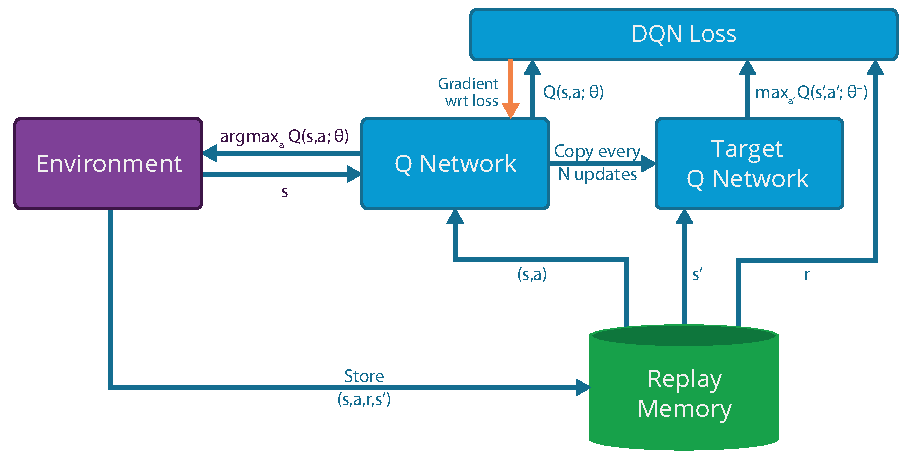
\includegraphics[width=\columnwidth]{DQNAgent_1}}
        \caption{The DQN algorithm is composed of three main components, the Q-network $(Q(s,a;\theta))$ that defines the behavior policy, the target Q-network $(Q(s,a;\theta^-))$ that is used to generate target Q values for the DQN loss term and the replay memory that the agent uses to sample random transitions for training the Q-network.}
        \label{DQN-figure}
    \end{center}
    \vskip -0.2in
\end{figure}

In the reinforcement learning (RL) paradigm, the agent interacts sequentially with an environment, with the goal of maximising cumulative rewards. At each step $t$ the agent observes state $s_t$, selects an action $a_t$, and receives a reward $r_t$. The agent's \emph{policy} $\pi(a | s)$ maps states to actions and defines its behavior. The goal of an RL agent is to maximize its expected total reward, where the rewards are discounted by a factor $\gamma \in [0,1]$ per time-step. Specifically, the \emph{return} at time $t$ is $R_t =\sum\limits_{t'=t}^{T} \gamma^{t'-t}r_{t'}$  where $T$ is the step when the episode terminates. The \emph{action-value function} $Q^\pi(s,a)$ is the expected return after observing state $s_t$ and taking an action under $a$ policy $\pi$, $Q^\pi(s,a) = \expect{}{R_t | s_t=s, a_t=a, \pi}$, and the \emph{optimal} action-value function is the maximum possible value that can be achieved by any policy, $Q^*(s,a) = \argmax{\pi}{Q^\pi(s,a)}$. The action-value function obeys a fundamental recursion known as the Bellman equation, $Q^*(s,a) = \expect{}{r + \gamma \ \max{a'}{Q^*(s',a')}}$. 

One of the core ideas behind reinforcement learning is to represent the action-value function using a function approximator such as a neural network, $Q(s,a) = Q(s,a; \theta)$. The parameters $\theta$ of the so-called \emph{Q-network} are optimized so as to approximately solve the Bellman equation. For example, the Q-learning algorithm iteratively updates the action-value function $Q(s,a; \theta)$ towards a sample of the Bellman target, $r + \gamma \ \max{a'}{Q(s',a'; \theta)}$. However, it is well-known that the Q-learning algorithm is highly unstable when combined with non-linear function approximators such as deep neural networks~\cite{tsitsiklis-convergence}. 

\subsection{Deep Q-Networks}
Recently, a new RL algorithm has been developed which is in practice much more stable when combined with deep Q-networks \cite{mnih2013atari,mnih-dqn-2015}. Like Q-learning, it iteratively solves the Bellman equation by adjusting the parameters of the Q-network towards the Bellman target. However, DQN, as shown in Figure~\ref{DQN-figure} differs from Q-learning in two ways. First, DQN uses experience replay \cite{lin1993reinforcement}. At each time-step $t$ during an agent's interaction with the environment it stores the experience tuple $e_t = (s_t, a_t, r_t, s_{t+1})$ into a replay memory $D_t = \{e_1, ..., e_t\}$. 

Second, DQN maintains two separate Q-networks $Q(s,a; \theta)$ and $Q(s,a; \theta^-)$ with current parameters $\theta$ and old parameters $\theta^-$ respectively. The current parameters $\theta$ may be updated many times per time-step, and are copied into the old parameters $\theta^-$ after $N$ iterations. At every update iteration $i$ the current parameters $\theta$ are updated so as to minimise the mean-squared Bellman error with respect to old parameters $\theta^-$, by optimizing the following loss function (DQN Loss),
%
\begin{small}
\begin{align}
L_i(\theta_i) = \expect{}{\left( r + \gamma \ \max{a'} Q(s', a'; \theta_i^-) - Q(s, a; \theta_i) \right)^2}
\end{align}
\end{small}
%
For each update $i$, a tuple of experience $(s,a,r,s') \sim U(D)$ (or a minibatch of such samples) is sampled uniformly from the replay memory $D$. For each sample (or minibatch), the current parameters $\theta$ are updated by a stochastic gradient descent algorithm. Specifically, $\theta$ is adjusted in the direction of the sample gradient $g_i$ of the loss with respect to $\theta$,
%
\begin{small}
\begin{align}
g_i = \left( r + \gamma \ \max{a'} Q(s', a'; \theta_i^-) - Q(s, a; \theta_i) \right) \nabla_{\theta_i} Q(s,a; \theta)
\label{eqn:dqngrad}
\end{align}
\end{small}
%
Finally, actions are selected at each time-step $t$ by an $\epsilon$-greedy behavior with respect to the current Q-network $Q(s,a;\theta)$.

%!TEX root = gorila_paper.tex
\section{Distributed Architecture}

\begin{figure*}[ht]
	%\vskip 0.2in
	\begin{center}
		\centerline{\includegraphics[width=\textwidth]{GorilaArchitecture2c}}
		\caption{The Gorila agent parallelises the training procedure by separating out learners, actors and parameter server. In a single experiment, several learner processes exist and they continuously send the gradients to parameter server and receive updated parameters. At the same time, independent actors can also in parallel accumulate experience and update their Q-networks from the parameter server. }
		\label{Gorila-figure}
	\end{center}
	\vskip -0.2in
\end{figure*}

\begin{algorithm}[t]
	\caption{Distributed DQN Algorithm}
	\label{alg:DistDQNAlgo}
	\begin{algorithmic}
		\STATE Initialise replay memory $D$ to size $P$.
		\STATE Initialise the training network for the action-value function $Q(s,a;\theta)$ with weights $\theta$ and target network $Q(s,a;\theta^-)$ with weights $\theta^- = \theta$.
		\FOR{$episode=1$ {\bfseries to} $M$}
		\STATE Initialise the start state to $s_{1}$.
		\STATE Update $\theta$ from parameters $\theta^+$ of the parameter server.
		\FOR{$t=1$ {\bfseries to} $T$}
		\STATE With probability $\epsilon$ take a random action $a_{t}$ or else $a_{t}$ = $\argmax{a}{Q(s, a ;\theta)}$.
		\STATE Execute the action in the environment and observe the reward $r_t$ and the next state $s_{t+1}$. Store $(s_t,a_t,r_t,s_{t+1})$ in $D$.
		\STATE Update $\theta$ from parameters $\theta^+$ of the parameter server.
		\STATE Sample random mini-batch from $D$. And for each tuple $(s_i,a_i,r_i,s_{i+1})$ set target $y_t$ as
		\IF{$s_{i+1} $ is $terminal$} 
		\STATE $y_t = r_i$
		\ELSE
		\STATE $y_t = r_i + \gamma \max{a'}{Q(s_{i+1}, a' ; \theta^{-})}$
		\ENDIF
		\STATE Calculate the loss $L_t = (y_t - Q(s_i, a_i ; \theta)^2)$.
		\STATE Compute gradients with respect to the network parameters $\theta$ using equation~\ref{eqn:dqngrad}.
		\STATE Send gradients to the parameter server.
		\STATE Every global $N$ steps sync $\theta^{-}$ with parameters $\theta^+$ from the parameter server.
		\ENDFOR
		\ENDFOR
	\end{algorithmic}
\end{algorithm}

We now introduce \emph{Gorila} (General Reinforcement Learning Architecture), a framework for massively distributed reinforcement learning. The Gorila architecture, shown in Figure~\ref{Gorila-figure} contains the following components:

{\bf Actors}. Any reinforcement learning agent must ultimately select actions $a_t$ to apply in its environment. We refer to this process as \emph{acting}. The Gorila architecture contains $N_{act}$ different actor processes, applied to $N_{act}$ corresponding instantiations of the same environment. Each actor $i$ generates its own trajectories of experience $s^i_1, a^i_1, r^i_1, ..., s^i_T, a^i_T, r^i_T$ within the environment, and as a result each actor may visit different parts of the state space. The quantity of experience that is generated by the actors after $T$ time-steps is approximately $TN_{act}$. Each actor contains a replica of the Q-network, which is used to determine behavior, for example using an $\epsilon$-greedy policy. The parameters of the Q-network are synchronized periodically from the parameter server.

{\bf Experience replay memory}. The experience tuples $e^i_t = (s^i_t, a^i_t, r^i_t, s^i_{t+1})$ generated by the actors are stored in a replay memory $D$. We consider two forms of experience replay memory. First, a \emph{local} replay memory stores each actor's experience $D^i_t =  \{ e^i_1, ..., e^i_t \}$ locally on that actor's machine. If a single machine has sufficient memory to store $M$ experience tuples, then the overall memory capacity becomes $MN_{act}$. Second, a \emph{global} replay memory aggregates the experience into a distributed database. In this approach the overall memory capacity is independent of $N_{act}$ and may be scaled as desired, at the cost of additional communication overhead.

{\bf Learners}. Gorila contains $N_{learn}$ learner processes. Each learner contains a replica of the Q-network and its job is to compute desired changes to the parameters of the Q-network. For each learner update $k$, a minibatch of experience tuples $e = (s,a,r,s')$ is sampled from either a local or global experience replay memory $D$ (see above). The learner applies an off-policy RL algorithm such as DQN \cite{mnih2013atari} to this minibatch of experience, in order to generate a gradient vector $g_i$.\footnote{The experience in the replay memory is generated by old behavior policies which are most likely different to the current behavior of the agent; therefore all updates must be performed off-policy \cite{sutton:book}.} The gradients $g_i$ are communicated to the parameter server; and the parameters of the Q-network are updated periodically from the parameter server. 

{\bf Parameter server}. Like DistBelief, the Gorila architecture uses a central parameter server to maintain a distributed representation of the Q-network $Q(s,a; \theta^+)$. The parameter vector $\theta^+$ is split disjointly across $N_{param}$ different machines. Each machine is responsible for applying gradient updates to a subset of the parameters. The parameter server receives gradients from the learners, and applies these gradients to modify the parameter vector $\theta^+$, using an asynchronous stochastic gradient descent algorithm. 

The Gorila architecture provides considerable flexibility in the number of ways an RL agent may be parallelized. It is possible to have parallel acting to generate large quantities of data into a global replay database, and then process that data with a single serial learner. In contrast, it is possible to have a single actor generating data into a local replay memory, and then have multiple learners process this data in parallel to learn as effectively as possible from this experience. However, to avoid any individual component from becoming a bottleneck, the Gorila architecture in general allows for arbitrary numbers of actors, learners, and parameter servers to both generate data, learn from that data, and update the model in a scalable and fully distributed fashion.

The simplest overall instantiation of Gorila, which we consider in our subsequent experiments, is the \emph{bundled} mode in which there is a one-to-one correspondence between actors, replay memory, and learners ($N_{act} = N_{learn}$). Each bundle has an actor generating experience, a local replay memory to store that experience, and a learner that updates parameters based on samples of experience from the local replay memory. The only communication between bundles is via parameters: the learners communicate their gradients to the parameter server; and the Q-networks in the actors and learners are periodically synchronized to the parameter server.

\subsection{Gorila DQN}

We now consider a specific instantiation of the Gorila architecture implementing the DQN algorithm.
As described in the previous section, the DQN algorithm utilizes two copies of the Q-network: a current Q-network with parameters $\theta$ and a target Q-network with parameters $\theta^-$.
The DQN algorithm is extended to the distributed implementation in Gorila as follows.
The parameter server maintains the current parameters $\theta^+$ and the actors and learners contain replicas of the current Q-network $Q(s,a;\theta)$ that are synchronized from the parameter server before every acting step.

The learner additionally maintains the target Q-network $Q(s,a;\theta^-)$.
The learner's target network is updated from the parameter server $\theta^+$ after every $N$ gradient updates in the central parameter server.

Note that $N$ is a global parameter that counts the total number of updates to the central parameter server rather than counting the updates from the local learner.

The learners generate gradients using the DQN gradient given in Equation~\ref{eqn:dqngrad}. However, the gradients are not applied directly, but instead communicated to the parameter server. The parameter server then applies the updates that are accumulated from many learners.

\subsection{Stability}
While the DQN training algorithm was designed to ensure stability of training neural networks with reinforcement learning, training using a large cluster of machines running multiple other tasks poses additional challenges.
The Gorila DQN implementation uses additional safeguards to ensure stability in the presence of disappearing nodes, slowdowns in network traffic, and slowdowns of individual machines.
One such safeguard is a parameter that determines the maximum time delay between the local parameters $\theta$ (the gradients $g_i$ are computed using $\theta$) and the parameters $\theta^+$ in the parameter server.

All gradients older than the threshold are discarded by the parameter server.  Additionally, each actor/learner keeps a running average and standard deviation of the absolute DQN loss for the data it sees and discards gradients with absolute loss higher than the mean plus several standard deviations.  Finally, we used the AdaGrad update rule ~\cite{duchi2011adaptive}.



% !TEX root = ../multi_task.tex

We evaluate the presented MTL method on a number of problems. First, we use MultiMNIST \citep{multi_mnist}, an MTL adaptation of MNIST \citep{mnist}. Next, we tackle multi-label classification on the CelebA dataset \citep{celeba} by considering each label as a distinct binary classification task. These problems include both classification and regression, with the number of tasks ranging from 2 to 40. Finally, we experiment with scene understanding, jointly tackling the tasks of semantic segmentation, instance segmentation, and depth estimation on the Cityscapes dataset \citep{cityscapes}. We discuss each experiment separately in the following subsections.

The baselines we consider are (i) \textbf{uniform scaling:} minimizing a uniformly weighted sum of loss functions \mbox{$\frac{1}{T}\sum_t \lL^t$}, \mbox{(ii) \textbf{single task:}} solving tasks independently, \mbox{(iii) \textbf{grid search:}} exhaustively trying various values from $\{ c^t \in [0,1] | \sum_t c^t = 1\}$ and optimizing for $\frac{1}{T}\sum_t c^t \lL^t$, \mbox{(iv) \textbf{\citet{Kendall2018}:}} using the uncertainty weighting proposed by \citet{Kendall2018}, and \mbox{(v) \textbf{GradNorm:}} using the normalization proposed by \citet{Chen2018}.



\subsection{MultiMNIST}
\label{sec:multi_mnist_exp}

Our initial experiments are on MultiMNIST, an MTL version of the MNIST dataset \citep{multi_mnist}. In order to convert digit classification into a multi-task problem, \citet{multi_mnist} overlaid multiple images together. We use a similar construction. For each image, a different one is chosen uniformly in random. Then one of these images is put at the top-left and the other one is at the bottom-right. The resulting tasks are: classifying the digit on the top-left (task-L) and classifying the digit on the bottom-right (task-R). We use 60K examples and directly apply existing single-task MNIST models. The MultiMNIST dataset is illustrated in the supplement.

We use the LeNet architecture \citep{mnist}. We treat all layers except the last as the representation function $g$ and put two fully-connected layers as task-specific functions (see the supplement for details). We visualize the performance profile as a scatter plot of accuracies on task-L and task-R in Figure~\ref{fig:multi_mnist_performance_curve}, and list the results in Table~\ref{tab:multi_mnist}.

In this setup, any static scaling results in lower accuracy than solving each task separately (the single-task baseline). The two tasks appear to compete for model capacity, since increase in the accuracy of one task results in decrease in the accuracy of the other. Uncertainty weighting \citep{Kendall2018} and GradNorm \citep{Chen2018} find solutions that are slightly better than grid search but distinctly worse than the single-task baseline. In contrast, our method finds a solution that efficiently utilizes the model capacity and yields accuracies that are as good as the single-task solutions. This experiment demonstrates the effectiveness of our method as well as the necessity of treating MTL as multi-objective optimization. Even after a large hyper-parameter search, \emph{any} scaling of tasks does not approach the effectiveness of our method.



\subsection{Multi-Label Classification}

\begin{figure}[t]
\includegraphics[width=\textwidth]{radar_full_new}
\vspace{1mm}
\caption{Radar charts of percentage error per attribute on CelebA \citep{celeba}. Lower is better. We divide attributes into two sets for legibility: easy on the left, hard on the right. Zoom in for details.}
\label{fig:multi_label_radar}
\end{figure}


\begin{wraptable}{r}{0.3\textwidth}
%\vspace{-4mm}
\captionof{table}{Mean of error per category of MTL algorithms in multi-label classification on CelebA \citep{celeba}.}
\begin{tabular}{r@{\hspace{2mm}}c@{}}
\toprule
& Average  \\
&  error \\
\midrule
Single task & $8.77$ \\
Uniform scaling & $9.62$ \\
\citealt{Kendall2018} & $9.53$ \\
GradNorm & $8.44$ \\
Ours & $\mathbf{8.25}$  \\
\bottomrule
\end{tabular}
\label{table:multi_label_bar}
%\vspace{-5mm}
\end{wraptable}

Next, we tackle multi-label classification. Given a set of attributes, multi-label classification calls for deciding whether each attribute holds for the input. We use the CelebA dataset \citep{celeba}, which includes 200K face images annotated with 40 attributes. Each attribute gives rise to a binary classification task and we cast this as a 40-way MTL problem. We use ResNet-18 \citep{resnet} without the final layer as a shared representation function, and attach a linear layer for each attribute (see the supplement for further details).


We plot the resulting error for each binary classification task as a radar chart in Figure~\ref{fig:multi_label_radar}. The average over them is listed in Table~\ref{table:multi_label_bar}. We skip grid search since it is not feasible over 40 tasks. Although uniform scaling is the norm in the multi-label classification literature, single-task performance is significantly better. Our method outperforms baselines for significant majority of tasks and achieves comparable performance in rest. This experiment also shows that our method remains effective when the number of tasks is high.


\subsection{Scene Understanding}

To evaluate our method in a more realistic setting, we use scene understanding. Given an RGB image, we solve three tasks: semantic segmentation (assigning pixel-level class labels), instance segmentation (assigning pixel-level instance labels), and monocular depth estimation (estimating continuous disparity per pixel). We follow the experimental procedure of \citet{Kendall2018} and use an encoder-decoder architecture. The encoder is based on ResNet-50 \citep{resnet} and is shared by all three tasks. The decoders are task-specific and are based on the pyramid pooling module \citep{pspnet} (see the supplement for further implementation details).

Since the output space of instance segmentation is unconstrained (the number of instances is not known in advance), we use a proxy problem as in \citet{Kendall2018}. For each pixel, we estimate the location of the center of mass of the instance that encompasses the pixel. These center votes can then be clustered to extract the instances. In our experiments, we directly report the MSE in the proxy task. Figure~\ref{fig:cityscapes_performance_profile} shows the performance profile for each pair of tasks, although we perform all experiments on all three tasks jointly. The pairwise performance profiles shown in Figure~\ref{fig:cityscapes_performance_profile} are simply 2D projections of the three-dimensional profile, presented this way for legibility. The results are also listed in Table~\ref{tab:cityscapes_results}.

MTL outperforms single-task accuracy, indicating that the tasks cooperate and help each other. Our method outperforms all baselines on all tasks.


\subsection{Role of the Approximation}

In order to understand the role of the approximation proposed in Section~\ref{sec:approximation}, we compare the final performance and training time of our algorithm with and without the presented approximation in Table~\ref{tab:approximation_tradeoff} (runtime measured on a single Titan Xp GPU). For a small number of tasks (3 for scene understanding), training time is reduced by 40\%. For the multi-label classification experiment (40 tasks), the presented approximation accelerates learning by a factor of 25.

On the accuracy side, we expect both methods to perform similarly as long as the full-rank assumption is satisfied. As expected, the accuracy of both methods is very similar. Somewhat surprisingly, our approximation results in slightly improved accuracy in all experiments. While counter-intuitive at first, we hypothesize that this is related to the use of SGD in the learning algorithm. Stability analysis in convex optimization suggests that if gradients are computed with an error $\hat{\nabla}_\btheta \mathcal{L}^t = \nabla_\btheta \mathcal{L}^t + \mathbf{e}^t$ ($\btheta$ corresponds to $\btheta^{sh}$ in (\ref{eq:kkt_opt})), as opposed to $\mathbf{Z}$ in the approximate problem in \ref{eq:approx}, the error in the solution is bounded as $\|\hat{\mathbf{\alpha}} - \mathbf{\alpha} \|_2 \leq \mathcal{O}(\max_t \|\mathbf{e}^t\|_2)$. Considering the fact that the gradients are computed over the full parameter set (millions of dimensions) for the original problem and over a smaller space for the approximation (batch size times representation which is in the thousands), the dimension of the error vector is significantly higher in the original problem. We expect the $l_2$ norm of such a random vector to depend on the dimension.

In summary, our quantitative analysis of the approximation suggests that (i) the approximation does not cause an accuracy drop and (ii) by solving an equivalent problem in a lower-dimensional space, our method achieves both better computational efficiency and higher stability.

  {\small
  \begin{table}[t]
%  \vspace{-4mm}
  \caption{Effect of the MGDA-UB approximation. We report the final accuracies as well as training times for our method with and without the approximation.}
  %\vspace{1mm}
  \centering
  \begin{tabular}{@{}r@{\hspace{3mm}}c@{\hspace{3mm}}c@{\hspace{2mm}}c@{\hspace{2mm}}c@{}c@{\hspace{5mm}}c@{\hspace{2mm}}c@{}}
  \toprule
  & \multicolumn{4}{c}{Scene understanding (3 tasks)} &  & \multicolumn{2}{c}{Multi-label (40 tasks)}  \\
  \cmidrule(r){2-5} \cmidrule(lr){7-8}
                  & Training & Segmentation & Instance  & Disparity      & & Training & Average \\
                 & time     &  mIoU [\%]       & error [px] & error [px] & & time (hour)      & error \\
  \midrule
  Ours (w/o approx.) & $38.6$ & $66.13$ & $10.28$ & $2.59$ & & $429.9$ & $8.33$ \\
  Ours & $\mathbf{23.3}$ & $\mathbf{66.63}$ & $\mathbf{10.25}$ & $\mathbf{2.54}$  & & $\mathbf{16.1}$ & $\mathbf{8.25}$ \\
  \bottomrule
  \end{tabular}
  %\vspace{-2mm}
  \label{tab:approximation_tradeoff}
  \end{table}}

\iffalse
\bibliography{ref.bib}
\fi

\section{Results}
We perform a variety of experiments across different tasks and neural network architectures in natural language processing as well as image classification. We report our experimental findings on language tasks in section~\ref{sec:NLP}, and image classification
in section~\ref{sec:image_class}. We illustrate that CBS schedules can alleviate sub-optimal initialization in section~\ref{sec:bad_init}. We follow the baseline training method for each task (for details please see Appendix~\ref{sec:training_outline}). 
Alongside testing/validation performance, we also report the number of training iterations (lower values are preferred).

\subsection{Language Results}\label{sec:NLP}

Language modeling is a challenging problem due to the complex and long-range interactions between distant words~\cite{merity2016pointer}.
One hope is that large/deep models might be able to 
capture these complex interactions, but large models easily overfit on these tasks and exhibit large gaps between training set and testing set performance. 
CBS schedules effectively help us avoid overfitting, and in addition snapshot ensembling enables even greater performance.

\begin{table}[!htbp]
\caption{\footnotesize Testing perplexity and number of parameter updates of L1 and L2 models on Penn 
Tree Bank (PTB) and WikiText~2 (WT2) datasets. The best perplexity and lowest number of 
updates are \textbf{bolded}. }
\label{tab:lm-results}
\centering
\begin{tabular}{lcc|cc|cc|cc} \toprule
  &\multicolumn{2}{c}{L1 on PTB}       &\multicolumn{2}{c}{L1 on WT2}    &\multicolumn{2}{c}{L2 on PTB} &\multicolumn{2}{c}{L2 on WT2}\\              
\midrule
Schedule    & {Per.}    & {\# Iters}    & {Per.}    & {\# Iters}    & {Per.}     & {\# Iters}   & {Per.}    & {\# Iters}      \\
\midrule
\Gc	BL\footnotemark	&	83.13	&	52k	&	96.41	&	116k	&	79.34	&	73k	&	99.69	&	164k	\\
\midrule
\Ga	CBS-10	&	80.49	&	49k	&	94.93	&	111k	&	79.37	&	83k	&	95.43	&	187k	\\
\Gc	CBS-5	&	80.78	&	49k	&	\textbf{94.31}	&	111k	&	78.61	&	73k	&	94.32	&	164k	\\
\Ga	CBS-1	&	81.56	&	49k	&	94.52	&	111k	&	77.56	&	69k	&	\textbf{91.78}	&	156k	\\
\midrule
\Gc	CBS-10-A	&	\textbf{80.28}	&	35k	&	95.91	&	79k	&	81.47	&	65k	&	95.28	&	146k	\\
\Ga	CBS-5-A	&	82.03	&	35k	&	95.23	&	79k	&	79.48	&	53k	&	93.63	&	118k	\\
\Gc	CBS-1-A	&	84.41	&	35k	&	95.66	&	79k	&	81.32	&	49k	&	93.19	&	111k	\\
\midrule
\Ga	CBS-10-T	&	80.49	&	49k	&	94.93	&	111k	&	79.42	&	83k	&	94.39	&	187k	\\
\Gc	CBS-5-T	&	80.94	&	53k	&	94.9	&	120k	&	78.95	&	63k	&	94.68	&	142k	\\
\Ga	CBS-1-T	&	81.82	&	46k	&	95.38	&	104k	&	\textbf{77.39}	&	65k	&	93.78	&	147k	\\
\bottomrule 
\end{tabular}
\end{table}

We evaluate a large variety of CBS schedules to positive results as shown in~\tref{tab:lm-results}. 
Results are measured in perplexity, a standard figure of merit for evaluating the quality of language models by measuring its prediction of the empirical distribution of words (lower perplexity value is better). 
As we can see, the best performing CBS schedules result in significant improvements in
perplexity (up to 7.91) over the baseline schedules and also offer reductions in the number of SGD training iterations (up to $33\%$). For example, CBS schedules achieve improvement of 7.91 perplexity improvement on WikiText~2 via CBS-1-T and reduce the SGD iterations from 164k to 111k via the CBS-1-A schedule.
Notice that almost all CBS schedules outperform the baseline schedule.
\begin{figure}[!htbp]
  \centering
\includegraphics[width=.4\textwidth]{fig/train_l2_ptb.pdf}
\includegraphics[width=.4\textwidth]{fig/test_l2_ptb.pdf}
  \caption{\footnotesize Training (left) and testing (right) perplexity as a function of iterations for the L2 model on PTB.}
  \label{fig:l2_ptb}
\end{figure}

\fref{fig:l2_ptb} shows the training and testing perplexity of the L2 model on PTB and WikiTest~2 as trained via the baseline schedule 
along with our best CBS schedule (from \tref{tab:lm-results}). Notice the cyclical spikes in training and testing perplexity. The peaks occur during  decreases in batch size, i.e., increases in noise scale, which could help to escape sub-optimal local minima, and the troughs occur during increases in batch size, i.e., decreases with noise scale.

In order to support our claim that CBS schedules are especially useful for counteracting overfitting, we conducted additional language modeling experiments on models L1', L2' with PTB and WT2 which use significantly lower dropout (0.2 and 0.3) than the original L1, L2 models (0.5 and 0.65). Because these models heavily overfit the training data, we report both the final testing perplexity as well as the best testing perplexity achieve during training. 
As seen in \tref{tab:lm-results-overfit} (in Appendix~\ref{sxn:app:additional results}), with L2' CBS yields improvements of a staggering 60.3 on final testing perplexity and 36.2 on best testing perplexity. CBS yields smaller improvements on L1' of 26.0 and 25.3, which are still much larger than the improvement achieved by CBS on L1 and L2. 


As mentioned above the goal of every cycle is to get an approximate MAP point. A very interesting idea
proposed in~\citep{huang2017snapshot} is to ensemble these MAP points by saving snapshots of the model
at the end of every cycle. We follow that strategy with the only difference that we use a batch size cycle
instead of cyclical learning rate proposed in~\citep{huang2017snapshot} due to higher parallelization opportunities for the former.
We perform experiments on snapshot ensembling with the L2 model with the respective best performing CBS schedules on PTB and WikiText~2 (CBS-1-T and CBS-1), as well as the fixed batch size baseline.
The CBS ensembles on PTB and WikiText~2 result in test set perplexity of 76.14 and 88.47, outperforming baseline ensembles on both datasets (76.52, 89.99 respectively) and CBS single models (77.39, 91.78 respectively).


To further explore the properties of cyclical batch size schedules, we also evaluate these schedules on natural language inference tasks, as shown in~\tref{tab:nli-results}. In our experiments, CBS schedules do not yield large performance improvements on models like E1 which exhibit smaller disparities between training and testing performance.
This is in line with our limitation in that CBS is more effective for models which tend to overfit. On the other hand, we see a large reduction in training 
iterations by up to 62\% which is due to higher effective batch size used in CBS than baseline.


\footnotetext{\citep{zaremba2014recurrent} reports testing perplexity of 82.7 and 78.4 
for L1 and L2 respectively on PTB, which we could not reproduce. The best perplexity and lowest number of updates are \textbf{bolded}.}

\begin{wraptable}{r}{7cm}
\caption{\footnotesize Validation accuracy and number of parameter updates of E1 on MultiNLI and SNLI 
datasets. The best accuracy and lowest number of updates are \textbf{bolded}. }
\label{tab:nli-results}
\centering
\begin{tabular}{lcc|cc} \toprule
  &\multicolumn{2}{c}{MultiNLI}       &\multicolumn{2}{c}{SNLI}    \\              
\midrule
Strategy    & {Acc.}    & {\# Iters}    & {Acc.}    & {\# Iters}    \\
\midrule
\Gc	BL	    &	72.87	&	123k	&	\textbf{86.86}	&	172k	\\
\Ga	CBS-1	&	\textbf{73.17}	&	64k	&	86.73   &   90k   \\
\Gc	CBS-2	&	73.07	&	71k	&	86.56   &   99k	\\
\Ga CBS-1-A &   72.23   & \textbf{48k}     & 86.26     & \textbf{67k}     \\
\Gc CBS-2-A &   72.04   & 57k     & 85.83     & 80k     \\
\bottomrule 
\end{tabular}
\end{wraptable}


\subsection{Image Classification Results}\label{sec:image_class}
We also test our CBS schedules on Cifar-10 and ImageNet. Table.~\ref{tab:cbs_cifar10} reports the testing accuracy and the number of training iterations for different models on Cifar-10. We see that the CBS schedules match baseline performance, but the number of training iterations used in CBS schedules is up to $2\times$ fewer. 

As seen in \fref{fig:wresnet_cifar10}, the training curves of CBS schedules also 
exhibit the aforementioned cyclical spikes both in training loss and testing 
accuracy. Similarly in the previously discussed language experiments, these spikes correspond to cycles in the CBS schedules and can 
be thought of as re-initializations of the neural network weights. We observe that CBS achieves similar performance to the baseline. 


\fref{fig:cbs_imagenet} shows the results of ResNet50 on ImageNet. The baseline trains in  $450k$ 
iterations and reaches $76.134\%$ validation accuracy. With CBS, the final validation accuracy is 
$76.336\%$, trained in $262k$ parameter updates.
CBS outperforms the baseline on both training loss and validation accuracy. 

We offer further support for the hypothesis that CBS schedules are more effective for overfitting neural networks with experiments on model C4, which achieves 94.35\% training 
accuracy 
and 55.55\% testing accuracy on Cifar-10. With CBS-15, we see 90.71\% training 
accuracy 
and 56.44\% testing accuracy, which is a larger improvement than that offered by CBS on convolutional models on Cifar-10.

We also explore combining CBS with the recent adversarial regularization proposed by~\cite{yao2018large}.
Combining CBS-15 on C2 with this strategy improves accuracy to $94.82\%$. This outperforms other schedules shown in  Table~\ref{tab:cbs_cifar10}.
Applying snapshot ensembling on C3 trained with CBS-15-2 leads to improved accuracy of $93.56\%$ as compared to $92.58\%$.
After ensembling ResNet50 on Imagenet with snapshots from the last two cycles, the performance increases to 76.401\% from 75.336\%.

\begin{table}[!htbp]
\caption{\footnotesize Accuracy and number of parameter updates of different models on Cifar-10. The best accuracy and lowest number of iterations are \textbf{bolded}.}
\label{tab:cbs_cifar10}
\centering
\begin{tabular}{lcc|lcc|lcc} \toprule
\multicolumn{3}{c}{AlexNet-like (C1)}  &\multicolumn{3}{c}{WResNet (C2)}  &\multicolumn{3}{c}{ResNet18 (C3)} \\              
\midrule
    {Strategy}                  & {Acc.} & {\# Iters}               &{Strategy}           & {Acc.} & {\# Iters}        &{Strategy}           & {Acc.} & {\# Iters}                     \\
    \midrule
\Gc  Baseline             &86.94            & 35k            & Baseline     &94.53   & 78k                   & Baseline      & \textbf{92.71}  & 63k          \\
\Ga  CBS-10-3          &86.83            & 20k               & CBS-15       &94.46   & 40k                   & CBS-10 & 92.47 & \textbf{32k}         \\
\Gc  CBS-15-2          &86.87            & 26k               & CBS-10-3     &\textbf{94.56}   & 45k          & CBS-5-3  & 92.45 & 37k        \\
\Ga  CBS-5-3           &\textbf{87.03}   & 20k      & CBS-5-3      &94.44   & 45k                   & CBS-15-2 & 92.58 & 48k         \\
\Gc  CBS-5-3-A         &86.75            & \textbf{15k}               & CBS-5-3-A    &94.34   & \textbf{33k}          & CBS-15-2-A & 92.27 & 39k             \\
     \bottomrule 
\end{tabular}
\end{table}



\begin{figure}[!htbp]
  \centering
\includegraphics[width=.4\textwidth]{fig/loss_c1.pdf}
\includegraphics[width=.4\textwidth]{fig/acc_c1.pdf}
  \caption{\footnotesize C2 model (WResNet) on Cifar-10. Training set loss (left), and testing set accuracy (right), evaluated as a function of epochs}

  \label{fig:wresnet_cifar10}
\end{figure}

\begin{figure}[!htbp]
  \centering
\includegraphics[width=.4\textwidth]{fig/loss_iter_I1.pdf}
\includegraphics[width=.4\textwidth]{fig/acc_iter_I1.pdf}
\includegraphics[width=.4\textwidth]{fig/loss_I1.pdf}
\includegraphics[width=.4\textwidth]{fig/acc_I1.pdf}

  \caption{\footnotesize I1 model (ResNet50) on ImageNet. Training set loss (left), and testing set accuracy (right), evaluated as a function of iterations (above) and epochs (below).}
  \label{fig:cbs_imagenet}
\end{figure}

\subsection{Sub-optimal Initialization}\label{sec:bad_init}
Various effective initialization methods~\cite{glorot2010understanding,he2015delving,saxe2013exact,mishkin2015all}
have been proposed previously; however, when presented with new architectures and new tasks,
initialization still needs to be explored empirically and often the final
performance varies greatly with different initializations. In this section, we test if
CBS schedules can alleviate the problem of sub-optimal initialization.

We test a Gaussian initialization with mean $0$ and standard deviation $0.1$ on 
an AlexNet-like model (C1). The baseline (BL) training follows the same setting as described in 
Appendix~\ref{sec:training_outline} and achieves final accuracy $84.27\%$. For CBS, we use cycle width of 10 with 3 steps.
In particular, CBS$_1$ denotes a constant learning rate, and achieves final accuracy $85.41\%$. CBS$_2$ decays the learning rate by a factor of 5 at
epoch 75 and achieves final accuracy $84.95\%$. 
We keep learning rate high during training because a high noise 
level helps $\theta$ escape sub-optimal local minima. 
Notice that all CBS methods achieve better generalization performance than the baseline.
\section{Conclusion}\label{sec:conclusion}
%\vspace{-.1in}
In this work, we apply the attentional encoder-decoder for the task of abstractive summarization with very promising results, outperforming state-of-the-art results significantly on two different datasets. Each of our proposed novel models addresses a specific problem in abstractive summarization, yielding further improvement in performance. We also propose a new dataset for multi-sentence summarization and establish benchmark numbers on it. As part of our future work, we plan to focus our efforts on this data and build more robust models for summaries consisting of multiple sentences.


%Our results strongly demonstrate that sequence-to-sequence models are extremely promising for summarization. Some of the other lessons we learned from our experiments are: (i) the LVT-trick is very useful for summarization as it improves training speed while not sacrificing performance; (ii) traditional methods such as vocabulary expansion and syntax-based features can boost performance of deep learning based models as well. As part of our ongoing work, we are investigating on ways to effectively generate rare words in the summary, which appears to be a glaring weakness in the existing models.  

\bibliographystyle{icml2015}
\bibliography{gorilabib}
\section{Positive Definiteness of~$K$}\label{sec:appendixA}
To show that the kernel~$K$ defined in~(\ref{eq:kernel}) is positive definite
(p.d.), we simply use elementary rules from the kernel literature described in
Sections 2.3.2 and 3.4.1 of~\cite{shawe2004}.  A linear combination of p.d. kernels with non-negative weights is also p.d. (see Proposition 3.22
of\cite{shawe2004}), and thus it is sufficient to show that for all $\z,\z'$
in~$\Omega$, the following kernel on $\Omega \to \HH$ is p.d.:
\begin{displaymath}
   (\varphi,\varphi') \mapsto \big\|\varphi(\z)\big\|_\HH  \normH{\varphi'(\z')} e^{-\frac{1}{2\sigma^2} \normH{\tildephi(\z)-\tildephi'(\z')}^2}.
\end{displaymath}
Specifically, it is also sufficient to
show that the following kernel on $\HH$ is p.d.:
\begin{displaymath}
   (\phi,\phi') \mapsto \big\|{\phi}\big\|_\HH  \normH{\phi'} e^{-\frac{1}{2\sigma^2} \normH{\frac{\phi}{\|\phi\|_\HH}-\frac{\phi'}{\|\phi'\|_\HH}}^2}.
\end{displaymath}
with the convention $\phi/\|\phi\|_\HH=0$ if~$\phi=0$.
This is a pointwise product of two kernels and is p.d. when each of the two
kernels is p.d. The first one is obviously p.d.: $(\phi,\phi') \mapsto
\|{\phi}\|_\HH  \normH{\phi'}$. The second one is a composition of the Gaussian
kernel---which is p.d.---, with feature maps $\phi/\|\phi\|_\HH$ of a
normalized linear kernel in~$\HH$.  This composition is p.d. according to
Proposition 3.22, item (v) of~\cite{shawe2004} since the normalization does
not remove the positive-definiteness property.

\section{List of Architectures Reported in the Experiments}\label{appendix:arch}
We present in details the architectures used in the paper in Table~\ref{table:arch}.
\begin{table}[hbtp]
   \centering
   \begin{tabular}{|*{9}{c|}}
      \hline
      Arch. & $N$ & $m_1$  & $p_1$  &  $\gamma_1$ & $m_2$ &  $p_2$ & $S$  &  $\sharp$ param\\
      \hline
      \hline
      \multicolumn{9}{|c|}{MNIST} \\
      \hline
      CKN-GM1 & 2 &  $1 \times 1$  &  12  & 2 &  $3 \times 3$ &  50 &  $4 \times 4$ & $5\,400$\\
      \hline
      CKN-GM2 & 2 &  $1 \times 1$  &  12  & 2 &  $3 \times 3$ &  400 &  $3 \times 3$& $43\,200$ \\
      \hline
      CKN-PM1 & 1 &  $5 \times 5$  &  200  & 2 &  - &  - &  $4 \times 4$  & $5\,000$ \\
      \hline
      CKN-PM2 & 2 &  $5 \times 5$  &  50  & 2 &  $2 \times 2$ &  200 &  $6 \times 6$ & $41\,250$ \\
      \hline
      \hline
      \multicolumn{9}{|c|}{CIFAR-10} \\
      \hline
      CKN-GM & 2 &  $1 \times 1$  &  12  & 2 &  $2 \times 2$ & 800 &  $4 \times 4$ & $38\,400$\\
      \hline
      CKN-PM & 2 &  $2 \times 2$  &  100  & 2 &  $2 \times 2$ &  800 &  $4 \times 4$ & $321\,200$\\
      \hline
      \hline
      \multicolumn{9}{|c|}{STL-10} \\
      \hline
      CKN-GM & 2 &  $1 \times 1$  &  12  & 2 &  $3 \times 3$ & 800 &  $4 \times 4$ & $86\,400$\\
      \hline
      CKN-PM & 2 &  $3 \times 3$  &  50  & 2 &  $3 \times 3$ &  800 &  $3 \times 3$ & $361\,350$\\
      \hline

   \end{tabular}
   \caption{List of architectures reported in the paper. $N$ is the number of layers; $p_1$ and~$p_2$ represent the number of filters are each layer; $m_1$ and~$m_2$ represent the size of the patches~$\NN_1$ and~$\NN_2$ that are of size~$m_1 \times m_1$ and~$m_2 \times m_2$ on their respective feature maps~$\zeta_1$ and~$\zeta_2$; $\gamma_1$ is the subsampling factor between layer 1 and layer 2; $S$ is the size of the output feature map, and the last column indicates the number of parameters that the network has to learn.}
   \label{table:arch}
\end{table}


\end{document} 
